% Options for packages loaded elsewhere
\PassOptionsToPackage{unicode}{hyperref}
\PassOptionsToPackage{hyphens}{url}
%
\documentclass[
]{book}
\usepackage{amsmath,amssymb}
\usepackage{iftex}
\ifPDFTeX
  \usepackage[T1]{fontenc}
  \usepackage[utf8]{inputenc}
  \usepackage{textcomp} % provide euro and other symbols
\else % if luatex or xetex
  \usepackage{unicode-math} % this also loads fontspec
  \defaultfontfeatures{Scale=MatchLowercase}
  \defaultfontfeatures[\rmfamily]{Ligatures=TeX,Scale=1}
\fi
\usepackage{lmodern}
\ifPDFTeX\else
  % xetex/luatex font selection
\fi
% Use upquote if available, for straight quotes in verbatim environments
\IfFileExists{upquote.sty}{\usepackage{upquote}}{}
\IfFileExists{microtype.sty}{% use microtype if available
  \usepackage[]{microtype}
  \UseMicrotypeSet[protrusion]{basicmath} % disable protrusion for tt fonts
}{}
\makeatletter
\@ifundefined{KOMAClassName}{% if non-KOMA class
  \IfFileExists{parskip.sty}{%
    \usepackage{parskip}
  }{% else
    \setlength{\parindent}{0pt}
    \setlength{\parskip}{6pt plus 2pt minus 1pt}}
}{% if KOMA class
  \KOMAoptions{parskip=half}}
\makeatother
\usepackage{xcolor}
\usepackage{color}
\usepackage{fancyvrb}
\newcommand{\VerbBar}{|}
\newcommand{\VERB}{\Verb[commandchars=\\\{\}]}
\DefineVerbatimEnvironment{Highlighting}{Verbatim}{commandchars=\\\{\}}
% Add ',fontsize=\small' for more characters per line
\usepackage{framed}
\definecolor{shadecolor}{RGB}{248,248,248}
\newenvironment{Shaded}{\begin{snugshade}}{\end{snugshade}}
\newcommand{\AlertTok}[1]{\textcolor[rgb]{0.94,0.16,0.16}{#1}}
\newcommand{\AnnotationTok}[1]{\textcolor[rgb]{0.56,0.35,0.01}{\textbf{\textit{#1}}}}
\newcommand{\AttributeTok}[1]{\textcolor[rgb]{0.13,0.29,0.53}{#1}}
\newcommand{\BaseNTok}[1]{\textcolor[rgb]{0.00,0.00,0.81}{#1}}
\newcommand{\BuiltInTok}[1]{#1}
\newcommand{\CharTok}[1]{\textcolor[rgb]{0.31,0.60,0.02}{#1}}
\newcommand{\CommentTok}[1]{\textcolor[rgb]{0.56,0.35,0.01}{\textit{#1}}}
\newcommand{\CommentVarTok}[1]{\textcolor[rgb]{0.56,0.35,0.01}{\textbf{\textit{#1}}}}
\newcommand{\ConstantTok}[1]{\textcolor[rgb]{0.56,0.35,0.01}{#1}}
\newcommand{\ControlFlowTok}[1]{\textcolor[rgb]{0.13,0.29,0.53}{\textbf{#1}}}
\newcommand{\DataTypeTok}[1]{\textcolor[rgb]{0.13,0.29,0.53}{#1}}
\newcommand{\DecValTok}[1]{\textcolor[rgb]{0.00,0.00,0.81}{#1}}
\newcommand{\DocumentationTok}[1]{\textcolor[rgb]{0.56,0.35,0.01}{\textbf{\textit{#1}}}}
\newcommand{\ErrorTok}[1]{\textcolor[rgb]{0.64,0.00,0.00}{\textbf{#1}}}
\newcommand{\ExtensionTok}[1]{#1}
\newcommand{\FloatTok}[1]{\textcolor[rgb]{0.00,0.00,0.81}{#1}}
\newcommand{\FunctionTok}[1]{\textcolor[rgb]{0.13,0.29,0.53}{\textbf{#1}}}
\newcommand{\ImportTok}[1]{#1}
\newcommand{\InformationTok}[1]{\textcolor[rgb]{0.56,0.35,0.01}{\textbf{\textit{#1}}}}
\newcommand{\KeywordTok}[1]{\textcolor[rgb]{0.13,0.29,0.53}{\textbf{#1}}}
\newcommand{\NormalTok}[1]{#1}
\newcommand{\OperatorTok}[1]{\textcolor[rgb]{0.81,0.36,0.00}{\textbf{#1}}}
\newcommand{\OtherTok}[1]{\textcolor[rgb]{0.56,0.35,0.01}{#1}}
\newcommand{\PreprocessorTok}[1]{\textcolor[rgb]{0.56,0.35,0.01}{\textit{#1}}}
\newcommand{\RegionMarkerTok}[1]{#1}
\newcommand{\SpecialCharTok}[1]{\textcolor[rgb]{0.81,0.36,0.00}{\textbf{#1}}}
\newcommand{\SpecialStringTok}[1]{\textcolor[rgb]{0.31,0.60,0.02}{#1}}
\newcommand{\StringTok}[1]{\textcolor[rgb]{0.31,0.60,0.02}{#1}}
\newcommand{\VariableTok}[1]{\textcolor[rgb]{0.00,0.00,0.00}{#1}}
\newcommand{\VerbatimStringTok}[1]{\textcolor[rgb]{0.31,0.60,0.02}{#1}}
\newcommand{\WarningTok}[1]{\textcolor[rgb]{0.56,0.35,0.01}{\textbf{\textit{#1}}}}
\usepackage{longtable,booktabs,array}
\usepackage{calc} % for calculating minipage widths
% Correct order of tables after \paragraph or \subparagraph
\usepackage{etoolbox}
\makeatletter
\patchcmd\longtable{\par}{\if@noskipsec\mbox{}\fi\par}{}{}
\makeatother
% Allow footnotes in longtable head/foot
\IfFileExists{footnotehyper.sty}{\usepackage{footnotehyper}}{\usepackage{footnote}}
\makesavenoteenv{longtable}
\usepackage{graphicx}
\makeatletter
\def\maxwidth{\ifdim\Gin@nat@width>\linewidth\linewidth\else\Gin@nat@width\fi}
\def\maxheight{\ifdim\Gin@nat@height>\textheight\textheight\else\Gin@nat@height\fi}
\makeatother
% Scale images if necessary, so that they will not overflow the page
% margins by default, and it is still possible to overwrite the defaults
% using explicit options in \includegraphics[width, height, ...]{}
\setkeys{Gin}{width=\maxwidth,height=\maxheight,keepaspectratio}
% Set default figure placement to htbp
\makeatletter
\def\fps@figure{htbp}
\makeatother
\setlength{\emergencystretch}{3em} % prevent overfull lines
\providecommand{\tightlist}{%
  \setlength{\itemsep}{0pt}\setlength{\parskip}{0pt}}
\setcounter{secnumdepth}{5}
\usepackage{booktabs}
\usepackage{amsthm}
\makeatletter
\def\thm@space@setup{%
  \thm@preskip=8pt plus 2pt minus 4pt
  \thm@postskip=\thm@preskip
}
\makeatother
\ifLuaTeX
  \usepackage{selnolig}  % disable illegal ligatures
\fi
\usepackage[]{natbib}
\bibliographystyle{apalike}
\usepackage{bookmark}
\IfFileExists{xurl.sty}{\usepackage{xurl}}{} % add URL line breaks if available
\urlstyle{same}
\hypersetup{
  pdftitle={Analyzing RCTs: A Cookbook},
  pdfauthor={Inge Christoffer Olsen},
  hidelinks,
  pdfcreator={LaTeX via pandoc}}

\title{Analyzing RCTs: A Cookbook}
\author{Inge Christoffer Olsen}
\date{2024-11-27}

\begin{document}
\maketitle

{
\setcounter{tocdepth}{1}
\tableofcontents
}
\chapter{Preface}\label{preface}

Placeholder

\section{Structure of the book}\label{structure-of-the-book}

\section{Acknowledgements}\label{acknowledgements}

\chapter{Introduction}\label{intro}

Placeholder

\section{Trial Flow}\label{trial-flow}

\section{Simulated dataset}\label{simulated-dataset}

\chapter{Continuous endpoints}\label{continuous-endpoints}

Placeholder

\section{Single follow-up}\label{single-follow-up}

\subsection{Stata code}\label{stata-code}

\subsection{R code}\label{r-code}

\subsection{Reporting}\label{reporting}

\section{Repeated follow-up}\label{repeated-follow-up}

\subsection{Simple model}\label{simple-model}

\subsection{Model with treatment-time interaction}\label{model-with-treatment-time-interaction}

\subsection{Model with treatment-time interaction and baseline information}\label{model-with-treatment-time-interaction-and-baseline-information}

\chapter{Dichotomous endpoints}\label{dichotomous-endpoints}

\section{Single follow-up}\label{single-follow-up-1}

For a single follow-up assessment of a dichotomous endpoint, the main method I use is a standard logistic regression. Then we can adjust for stratification factors in the randomisation in addition to other pre-specified covariates, both categorical and continuous. In the simulated example, we define that the primary outcome is the dichotomous categorical outcome at time 3. Note that usually the baseline status of all patients are negative for the outcome, so adjusting for baseline is not necessary.

\subsection{Stata code}\label{stata-code-1}

\begin{Shaded}
\begin{Highlighting}[]
\KeywordTok{use} \StringTok{"stata/rct"}\NormalTok{, }\KeywordTok{clear} 
\KeywordTok{tabulate}\NormalTok{ catout trt }\KeywordTok{if}\NormalTok{ time == 3, column}
\KeywordTok{logistic}\NormalTok{ catout i.trt i.site covar  }\KeywordTok{if}\NormalTok{ time==3, coef}
\end{Highlighting}
\end{Shaded}

\begin{verbatim}
(all strata combined)


+-------------------+
| Key               |
|-------------------|
|     frequency     |
| column percentage |
+-------------------+

Categorica |       Treatment
 l outcome |   Placebo     Active |     Total
-----------+----------------------+----------
  Negative |         9         22 |        31 
           |     18.00      45.83 |     31.63 
-----------+----------------------+----------
  Positive |        41         26 |        67 
           |     82.00      54.17 |     68.37 
-----------+----------------------+----------
     Total |        50         48 |        98 
           |    100.00     100.00 |    100.00 


Logistic regression                                     Number of obs =     98
                                                        LR chi2(5)    =  48.59
                                                        Prob > chi2   = 0.0000
Log likelihood = -36.862204                             Pseudo R2     = 0.3973

------------------------------------------------------------------------------
      catout | Coefficient  Std. err.      z    P>|z|     [95% conf. interval]
-------------+----------------------------------------------------------------
         trt |
     Active  |  -2.890301   .7850252    -3.68   0.000    -4.428922   -1.351679
             |
        site |
          2  |   .7783404   .8580245     0.91   0.364    -.9033566    2.460037
          3  |   1.423791   .7786531     1.83   0.067    -.1023412    2.949923
          4  |   .0253234   .8082887     0.03   0.975    -1.558893     1.60954
             |
       covar |   1.001078   .2329461     4.30   0.000     .5445124    1.457644
       _cons |  -2.463577   .8925892    -2.76   0.006     -4.21302   -.7141344
------------------------------------------------------------------------------
\end{verbatim}

Note that the use the \texttt{coef} option to get the log odds ratio estimates.

\subsection{R code}\label{r-code-1}

\begin{Shaded}
\begin{Highlighting}[]
\NormalTok{rct }\OtherTok{\textless{}{-}} \FunctionTok{read\_dta}\NormalTok{(}\StringTok{"stata/rct.dta"}\NormalTok{) }\SpecialCharTok{\%\textgreater{}\%} 
  \FunctionTok{modify\_at}\NormalTok{(}\FunctionTok{c}\NormalTok{(}\StringTok{"trt"}\NormalTok{,}\StringTok{"catout"}\NormalTok{), haven}\SpecialCharTok{::}\NormalTok{as\_factor, }\AttributeTok{levels =} \StringTok{"labels"}\NormalTok{) }\SpecialCharTok{\%\textgreater{}\%} 
  \FunctionTok{modify\_at}\NormalTok{(}\FunctionTok{c}\NormalTok{(}\StringTok{"site"}\NormalTok{,}\StringTok{"time"}\NormalTok{), haven}\SpecialCharTok{::}\NormalTok{as\_factor)}
\NormalTok{rct }\SpecialCharTok{\%\textgreater{}\%} 
  \FunctionTok{filter}\NormalTok{(time}\SpecialCharTok{==}\DecValTok{3}\NormalTok{) }\SpecialCharTok{\%\textgreater{}\%}
  \FunctionTok{glm}\NormalTok{(catout }\SpecialCharTok{\textasciitilde{}}\NormalTok{ trt }\SpecialCharTok{+}\NormalTok{ site }\SpecialCharTok{+}\NormalTok{ covar , }\AttributeTok{data=}\NormalTok{., }\AttributeTok{family =}\NormalTok{ binomial) }\SpecialCharTok{\%\textgreater{}\%}
\NormalTok{  summary}
\end{Highlighting}
\end{Shaded}

\begin{verbatim}

Call:
glm(formula = catout ~ trt + site + covar, family = binomial, 
    data = .)

Coefficients:
            Estimate Std. Error z value Pr(>|z|)    
(Intercept) -2.46358    0.89259  -2.760 0.005780 ** 
trtActive   -2.89030    0.78502  -3.682 0.000232 ***
site2        0.77834    0.85802   0.907 0.364337    
site3        1.42379    0.77865   1.829 0.067470 .  
site4        0.02532    0.80829   0.031 0.975007    
covar        1.00108    0.23295   4.297 1.73e-05 ***
---
Signif. codes:  0 '***' 0.001 '**' 0.01 '*' 0.05 '.' 0.1 ' ' 1

(Dispersion parameter for binomial family taken to be 1)

    Null deviance: 122.318  on 97  degrees of freedom
Residual deviance:  73.724  on 92  degrees of freedom
AIC: 85.724

Number of Fisher Scoring iterations: 6
\end{verbatim}

Not surprisingly, the estimates are identical.

\subsection{Reporting}\label{reporting-1}

Reporting for dichotomous endpoints is a bit tricky. The natural estimates from a logistic regression is odds and odds ratios, but these are less interpretable than risk differences or relative risk. As New England Journal of Medicine states in their Statistical Guidelines: ``Odds ratios should be avoided, as they may overestimate the relative risks in many settings and be misinterpreted.'' Fortunately, both Stata and R can estimate adjusted risk differences and relative risks from logistic regressions.

\subsubsection{Stata code}\label{stata-code-2}

First we compute the average prediced marginal probabilities. Basically this is done by calculating the predicted probability of a positive outcome for each patient, under both treatments, and then averaging. The standard errors are computed by the delta method.

\begin{Shaded}
\begin{Highlighting}[]
\KeywordTok{use} \StringTok{"stata/rct"}\NormalTok{, }\KeywordTok{clear} 
\KeywordTok{quietly} \KeywordTok{logistic}\NormalTok{ catout i.trt i.site covar  }\KeywordTok{if}\NormalTok{ time==3, coef}
\NormalTok{margins trt}
\end{Highlighting}
\end{Shaded}

\begin{verbatim}
(all strata combined)



Predictive margins                                          Number of obs = 98
Model VCE: OIM

Expression: Pr(catout), predict()

------------------------------------------------------------------------------
             |            Delta-method
             |     Margin   std. err.      z    P>|z|     [95% conf. interval]
-------------+----------------------------------------------------------------
         trt |
    Placebo  |   .8499905   .0387218    21.95   0.000     .7740972    .9258839
     Active  |   .5111833   .0533918     9.57   0.000     .4065374    .6158293
------------------------------------------------------------------------------
\end{verbatim}

The adjusted risk difference is calculated similarly.

\begin{Shaded}
\begin{Highlighting}[]
\KeywordTok{use} \StringTok{"stata/rct"}\NormalTok{, }\KeywordTok{clear} 
\KeywordTok{quietly} \KeywordTok{logistic}\NormalTok{ catout i.trt i.site covar  }\KeywordTok{if}\NormalTok{ time==3, coef}
\NormalTok{margins, }\KeywordTok{dydx}\NormalTok{(trt)}
\end{Highlighting}
\end{Shaded}

\begin{verbatim}
(all strata combined)



Average marginal effects                                    Number of obs = 98
Model VCE: OIM

Expression: Pr(catout), predict()
dy/dx wrt:  1.trt

------------------------------------------------------------------------------
             |            Delta-method
             |      dy/dx   std. err.      z    P>|z|     [95% conf. interval]
-------------+----------------------------------------------------------------
         trt |
     Active  |  -.3388072   .0661086    -5.13   0.000    -.4683777   -.2092367
------------------------------------------------------------------------------
Note: dy/dx for factor levels is the discrete change from the base level.
\end{verbatim}

We see that the risk difference is the difference of the estimated marginal probabilities we computed previously.

The relative risk is a bit more difficult to calculate, but not much. It uses the \texttt{nlcom} method to compute non-linear combinations of estimates.

\begin{Shaded}
\begin{Highlighting}[]
\KeywordTok{use} \StringTok{"stata/rct"}\NormalTok{, }\KeywordTok{clear} 
\KeywordTok{quietly} \KeywordTok{logistic}\NormalTok{ catout i.trt i.site covar  }\KeywordTok{if}\NormalTok{ time==3, coef}
\KeywordTok{quietly}\NormalTok{ margins trt, }\KeywordTok{post}
\NormalTok{margins, coeflegend}
\KeywordTok{nlcom}\NormalTok{ (ratio1: (\_b[1.trt]/\_b[0bn.trt]))}
\end{Highlighting}
\end{Shaded}

\begin{verbatim}
(all strata combined)




Predictive margins                                          Number of obs = 98
Model VCE: OIM

Expression: Pr(catout), predict()

------------------------------------------------------------------------------
             |     Margin   Legend
-------------+----------------------------------------------------------------
         trt |
    Placebo  |   .8499905  _b[0bn.trt]
     Active  |   .5111833  _b[1.trt]
------------------------------------------------------------------------------

      ratio1: (_b[1.trt]/_b[0bn.trt])

------------------------------------------------------------------------------
             | Coefficient  Std. err.      z    P>|z|     [95% conf. interval]
-------------+----------------------------------------------------------------
      ratio1 |   .6013989   .0686524     8.76   0.000     .4668426    .7359552
------------------------------------------------------------------------------
\end{verbatim}

The trick is to know what goes into the \_b{[}{]}-brackets, which will be revealed using the `coeflegend´-option. Note that I do not know the properties of this estimator, and it might be clever to check the estimates using bootstrap.

Some journals require calculation of the number needed to treat (NNT), at least if the confidence interval of the adjusted risk difference does not include zero (for which the NNT is undefined). This is simply done by inverting the adjusted risk difference estimate (both point estimate and the confidence limits).

\subsubsection{R code}\label{r-code-2}

The average predicted marginal probabilities was previously not easily computed in R, but with the emergence of the very nice \texttt{marginaleffects}-package, this is now much easier:

\begin{Shaded}
\begin{Highlighting}[]
\NormalTok{mod }\OtherTok{\textless{}{-}}\NormalTok{ rct }\SpecialCharTok{\%\textgreater{}\%} 
  \FunctionTok{filter}\NormalTok{(time }\SpecialCharTok{==} \DecValTok{3}\NormalTok{) }\SpecialCharTok{\%\textgreater{}\%}
  \FunctionTok{glm}\NormalTok{(catout }\SpecialCharTok{\textasciitilde{}}\NormalTok{ trt }\SpecialCharTok{+}\NormalTok{ site }\SpecialCharTok{+}\NormalTok{ covar , }\AttributeTok{data=}\NormalTok{., }\AttributeTok{family =}\NormalTok{ binomial)}

\NormalTok{mod }\SpecialCharTok{\%\textgreater{}\%}
  \FunctionTok{avg\_predictions}\NormalTok{(}\AttributeTok{variables =} \FunctionTok{list}\NormalTok{(}\AttributeTok{trt =} \FunctionTok{c}\NormalTok{(}\StringTok{"Active"}\NormalTok{, }\StringTok{"Placebo"}\NormalTok{)), }\AttributeTok{type =} \StringTok{"response"}\NormalTok{) }
\end{Highlighting}
\end{Shaded}

\begin{verbatim}

     trt Estimate Std. Error     z Pr(>|z|)     S 2.5 % 97.5 %
 Active     0.511     0.0534  9.57   <0.001  69.7 0.407  0.616
 Placebo    0.850     0.0387 21.95   <0.001 352.4 0.774  0.926

Columns: trt, estimate, std.error, statistic, p.value, s.value, conf.low, conf.high 
Type:  response 
\end{verbatim}

We notice that the estimates are equal to the Stata output..

Another option is to bootstrap the predicted marginal predictions:

\begin{Shaded}
\begin{Highlighting}[]
\FunctionTok{library}\NormalTok{(boot)}

\NormalTok{ fpred }\OtherTok{\textless{}{-}} \ControlFlowTok{function}\NormalTok{(formula, data, indices)\{}
\NormalTok{   d }\OtherTok{\textless{}{-}}\NormalTok{ data[indices,]}
\NormalTok{   fit }\OtherTok{\textless{}{-}} \FunctionTok{glm}\NormalTok{(formula, }\AttributeTok{data =}\NormalTok{ d, }\AttributeTok{family =}\NormalTok{ binomial)}
\NormalTok{   pred }\OtherTok{\textless{}{-}} \FunctionTok{prediction}\NormalTok{(fit,}\AttributeTok{data =}\NormalTok{ d, }\AttributeTok{at =} \FunctionTok{list}\NormalTok{(}\AttributeTok{trt =} \FunctionTok{c}\NormalTok{(}\StringTok{"Active"}\NormalTok{, }\StringTok{"Placebo"}\NormalTok{))) }\SpecialCharTok{\%\textgreater{}\%}
\NormalTok{     as\_tibble }\SpecialCharTok{\%\textgreater{}\%}
     \FunctionTok{group\_by}\NormalTok{(trt) }\SpecialCharTok{\%\textgreater{}\%}
     \FunctionTok{summarise}\NormalTok{(}\AttributeTok{mean =} \FunctionTok{mean}\NormalTok{(fitted)) }\SpecialCharTok{\%\textgreater{}\%}
     \FunctionTok{ungroup}\NormalTok{() }\SpecialCharTok{\%\textgreater{}\%}
     \FunctionTok{mutate}\NormalTok{(}\AttributeTok{name =} \FunctionTok{paste0}\NormalTok{(trt)) }\SpecialCharTok{\%\textgreater{}\%}
     \FunctionTok{select}\NormalTok{(name,mean) }\SpecialCharTok{\%\textgreater{}\%}
     \FunctionTok{spread}\NormalTok{(name,mean) }\SpecialCharTok{\%\textgreater{}\%}
\NormalTok{     as\_vector}
   \FunctionTok{return}\NormalTok{(pred)}
\NormalTok{ \}}
 
\NormalTok{ data }\OtherTok{\textless{}{-}} \FunctionTok{filter}\NormalTok{(rct, time }\SpecialCharTok{==} \DecValTok{3}\NormalTok{)}
\NormalTok{ result }\OtherTok{\textless{}{-}} \FunctionTok{boot}\NormalTok{(}\AttributeTok{data =}\NormalTok{ data, }
                \AttributeTok{statistic =}\NormalTok{ fpred, }
                \AttributeTok{R =} \DecValTok{10000}\NormalTok{, }
                \AttributeTok{formula =}\NormalTok{ catout }\SpecialCharTok{\textasciitilde{}}\NormalTok{ trt }\SpecialCharTok{+}\NormalTok{ site }\SpecialCharTok{+}\NormalTok{ covar,}
                \AttributeTok{parallel =} \StringTok{"multicore"}\NormalTok{,}
                \AttributeTok{ncpus =} \DecValTok{4}\NormalTok{) }\SpecialCharTok{\%\textgreater{}\%}
   \FunctionTok{tidy}\NormalTok{(}\AttributeTok{conf.int =} \ConstantTok{TRUE}\NormalTok{) }
\end{Highlighting}
\end{Shaded}

\begin{verbatim}
Error in prediction(fit, data = d, at = list(trt = c("Active", "Placebo"))): could not find function "prediction"
\end{verbatim}

\begin{Shaded}
\begin{Highlighting}[]
\NormalTok{ result }\SpecialCharTok{\%\textgreater{}\%}
   \FunctionTok{select}\NormalTok{(}\SpecialCharTok{{-}}\NormalTok{bias) }\SpecialCharTok{\%\textgreater{}\%}
\NormalTok{   knitr}\SpecialCharTok{::}\FunctionTok{kable}\NormalTok{(}\AttributeTok{digits =} \DecValTok{3}\NormalTok{)}
\end{Highlighting}
\end{Shaded}

\begin{verbatim}
Error in eval(expr, envir, enclos): object 'result' not found
\end{verbatim}

We see that the estimates are identical to the Stata estimates, although the standard errors and confidence limits are a bit different. But I actually think the bootstrap estimates are better.

The estimated marginal risk difference in R is computed using the \texttt{marginaleffects}-package again.

\begin{Shaded}
\begin{Highlighting}[]
\NormalTok{ rlogistic }\OtherTok{\textless{}{-}}\NormalTok{ rct }\SpecialCharTok{\%\textgreater{}\%} 
  \FunctionTok{filter}\NormalTok{(time}\SpecialCharTok{==}\DecValTok{3}\NormalTok{) }\SpecialCharTok{\%\textgreater{}\%}
  \FunctionTok{glm}\NormalTok{(catout }\SpecialCharTok{\textasciitilde{}}\NormalTok{ trt }\SpecialCharTok{+}\NormalTok{ site }\SpecialCharTok{+}\NormalTok{ covar , }\AttributeTok{data=}\NormalTok{., }\AttributeTok{family =}\NormalTok{ binomial)}


\NormalTok{  rlogistic }\SpecialCharTok{\%\textgreater{}\%} 
    \FunctionTok{avg\_comparisons}\NormalTok{(}\AttributeTok{variables =} \FunctionTok{list}\NormalTok{(}\AttributeTok{trt =} \FunctionTok{c}\NormalTok{(}\StringTok{"Active"}\NormalTok{, }\StringTok{"Placebo"}\NormalTok{)), }\AttributeTok{type =} \StringTok{"response"}\NormalTok{)}
\end{Highlighting}
\end{Shaded}

\begin{verbatim}

 Term         Contrast Estimate Std. Error    z Pr(>|z|)    S 2.5 % 97.5 %
  trt Placebo - Active    0.339     0.0661 5.13   <0.001 21.7 0.209  0.468

Columns: term, contrast, estimate, std.error, statistic, p.value, s.value, conf.low, conf.high 
Type:  response 
\end{verbatim}

We see that the estimates are identical to the Stata estimates.

The relative risk is very easily computed in R using the \texttt{marginaleffects}-package:

\begin{Shaded}
\begin{Highlighting}[]
\NormalTok{ rlogistic }\OtherTok{\textless{}{-}}\NormalTok{ rct }\SpecialCharTok{\%\textgreater{}\%} 
  \FunctionTok{filter}\NormalTok{(time}\SpecialCharTok{==}\DecValTok{3}\NormalTok{) }\SpecialCharTok{\%\textgreater{}\%}
  \FunctionTok{glm}\NormalTok{(catout }\SpecialCharTok{\textasciitilde{}}\NormalTok{ trt }\SpecialCharTok{+}\NormalTok{ site }\SpecialCharTok{+}\NormalTok{ covar , }\AttributeTok{data=}\NormalTok{., }\AttributeTok{family =}\NormalTok{ binomial)}


\NormalTok{  rlogistic }\SpecialCharTok{\%\textgreater{}\%} 
    \FunctionTok{avg\_comparisons}\NormalTok{(}\AttributeTok{variables =} \FunctionTok{list}\NormalTok{(}\AttributeTok{trt =} \FunctionTok{c}\NormalTok{(}\StringTok{"Active"}\NormalTok{, }\StringTok{"Placebo"}\NormalTok{)), }\AttributeTok{type =} \StringTok{"response"}\NormalTok{, }\AttributeTok{comparison =} \StringTok{"ratioavg"}\NormalTok{)}
\end{Highlighting}
\end{Shaded}

\begin{verbatim}

 Term                     Contrast Estimate Std. Error    z Pr(>|z|)    S 2.5 %
  trt mean(Placebo) / mean(Active)     1.66       0.19 8.76   <0.001 58.8  1.29
 97.5 %
   2.03

Columns: term, contrast, estimate, std.error, statistic, p.value, s.value, conf.low, conf.high, predicted_lo, predicted_hi, predicted 
Type:  response 
\end{verbatim}

The estimate is the inverse of the Stata estimate, and the confidence limits are very similar. There is probably a slight difference in how these are computed.

This is possible to do also by bootstrapping, but it is a bit more complicated:

\begin{Shaded}
\begin{Highlighting}[]
\FunctionTok{library}\NormalTok{(boot)}
\FunctionTok{library}\NormalTok{(prediction)}


\NormalTok{ fpred }\OtherTok{\textless{}{-}} \ControlFlowTok{function}\NormalTok{(formula, data, indices)\{}
\NormalTok{   d }\OtherTok{\textless{}{-}}\NormalTok{ data[indices,]}
\NormalTok{   fit }\OtherTok{\textless{}{-}} \FunctionTok{glm}\NormalTok{(formula, }\AttributeTok{data =}\NormalTok{ d, }\AttributeTok{family =}\NormalTok{ binomial)}
\NormalTok{   pred }\OtherTok{\textless{}{-}} \FunctionTok{prediction}\NormalTok{(fit,}\AttributeTok{data =}\NormalTok{ d, }\AttributeTok{at =} \FunctionTok{list}\NormalTok{(}\AttributeTok{trt =} \FunctionTok{c}\NormalTok{(}\StringTok{"Active"}\NormalTok{, }\StringTok{"Placebo"}\NormalTok{))) }\SpecialCharTok{\%\textgreater{}\%}
\NormalTok{     as\_tibble }\SpecialCharTok{\%\textgreater{}\%}
     \FunctionTok{group\_by}\NormalTok{(trt) }\SpecialCharTok{\%\textgreater{}\%}
     \FunctionTok{summarise}\NormalTok{(}\AttributeTok{mean =} \FunctionTok{mean}\NormalTok{(fitted)) }\SpecialCharTok{\%\textgreater{}\%}
     \FunctionTok{ungroup}\NormalTok{() }\SpecialCharTok{\%\textgreater{}\%}
     \FunctionTok{mutate}\NormalTok{(}\AttributeTok{name =} \FunctionTok{paste0}\NormalTok{(trt)) }\SpecialCharTok{\%\textgreater{}\%}
     \FunctionTok{select}\NormalTok{(name,mean) }\SpecialCharTok{\%\textgreater{}\%}
     \FunctionTok{spread}\NormalTok{(name,mean) }\SpecialCharTok{\%\textgreater{}\%}
\NormalTok{     as\_vector}
   \FunctionTok{return}\NormalTok{(pred[}\StringTok{"Active"}\NormalTok{]}\SpecialCharTok{/}\NormalTok{pred[}\StringTok{"Placebo"}\NormalTok{])}
\NormalTok{ \}}
 
\NormalTok{ data }\OtherTok{\textless{}{-}} \FunctionTok{filter}\NormalTok{(rct, time }\SpecialCharTok{==} \DecValTok{3}\NormalTok{)}
\NormalTok{ result }\OtherTok{\textless{}{-}} \FunctionTok{boot}\NormalTok{(}\AttributeTok{data =}\NormalTok{ data, }
                \AttributeTok{statistic =}\NormalTok{ fpred, }
                \AttributeTok{R =} \DecValTok{10000}\NormalTok{, }
                \AttributeTok{formula =}\NormalTok{ catout }\SpecialCharTok{\textasciitilde{}}\NormalTok{ trt }\SpecialCharTok{+}\NormalTok{ site }\SpecialCharTok{+}\NormalTok{ covar,}
                \AttributeTok{parallel =} \StringTok{"multicore"}\NormalTok{,}
                \AttributeTok{ncpus =} \DecValTok{4}\NormalTok{) }\SpecialCharTok{\%\textgreater{}\%}
   \FunctionTok{tidy}\NormalTok{(}\AttributeTok{conf.int =} \ConstantTok{TRUE}\NormalTok{) }
 
\NormalTok{ result }\SpecialCharTok{\%\textgreater{}\%}
   \FunctionTok{select}\NormalTok{(}\SpecialCharTok{{-}}\NormalTok{bias) }\SpecialCharTok{\%\textgreater{}\%}
\NormalTok{   knitr}\SpecialCharTok{::}\FunctionTok{kable}\NormalTok{(}\AttributeTok{digits =} \DecValTok{3}\NormalTok{)}
\end{Highlighting}
\end{Shaded}

\begin{tabular}{l|r|r|r|r}
\hline
term & statistic & std.error & conf.low & conf.high\\
\hline
Active & 0.601 & 0.081 & 0.446 & 0.763\\
\hline
\end{tabular}

\section{Repeated follow-up}\label{repeated-follow-up-1}

When there are repeated dichotomous endpoints, there are usually two methods available, either the generalized estimating equations method or the generalized mixed model method. I prefer the mixed model approach because it has better missing data properties, and I like that the parameter estimates are interpretable conditional on the subject. In my mind it is more aligned to a causal interpretation. I will show how to do the mixed logistic regression model. We skip the simple model and go straight to a model with treatment-time interaction. Note that usually a dichotomous endpoint all have the same value at baseline (all subjects are in the same state), thus we rarely include the baseline. The model is a simple random intercept model, but it could of course also be expanded to a random intercept and slope model.

\section{Treatment-time interaction model}\label{treatment-time-interaction-model}

In Stata, the model is coded as:

\begin{Shaded}
\begin{Highlighting}[]
\KeywordTok{use} \StringTok{"stata/rct"}\NormalTok{, }\KeywordTok{clear} 
\KeywordTok{bysort}\NormalTok{ time: }\KeywordTok{tabulate}\NormalTok{ catout trt, column}
\NormalTok{melogit catout i.trt i.site covar i.time i.trt\#i.time }\KeywordTok{if}\NormalTok{ time != 0 || pid: }
\end{Highlighting}
\end{Shaded}

\begin{verbatim}
(all strata combined)


-------------------------------------------------------------------------------
-> time = 0

+-------------------+
| Key               |
|-------------------|
|     frequency     |
| column percentage |
+-------------------+

Categorica |       Treatment
 l outcome |   Placebo     Active |     Total
-----------+----------------------+----------
  Negative |        50         48 |        98 
           |    100.00     100.00 |    100.00 
-----------+----------------------+----------
     Total |        50         48 |        98 
           |    100.00     100.00 |    100.00 

-------------------------------------------------------------------------------
-> time = 1

+-------------------+
| Key               |
|-------------------|
|     frequency     |
| column percentage |
+-------------------+

Categorica |       Treatment
 l outcome |   Placebo     Active |     Total
-----------+----------------------+----------
  Negative |        24         32 |        56 
           |     48.00      66.67 |     57.14 
-----------+----------------------+----------
  Positive |        26         16 |        42 
           |     52.00      33.33 |     42.86 
-----------+----------------------+----------
     Total |        50         48 |        98 
           |    100.00     100.00 |    100.00 

-------------------------------------------------------------------------------
-> time = 2

+-------------------+
| Key               |
|-------------------|
|     frequency     |
| column percentage |
+-------------------+

Categorica |       Treatment
 l outcome |   Placebo     Active |     Total
-----------+----------------------+----------
  Negative |        12         29 |        41 
           |     24.00      60.42 |     41.84 
-----------+----------------------+----------
  Positive |        38         19 |        57 
           |     76.00      39.58 |     58.16 
-----------+----------------------+----------
     Total |        50         48 |        98 
           |    100.00     100.00 |    100.00 

-------------------------------------------------------------------------------
-> time = 3

+-------------------+
| Key               |
|-------------------|
|     frequency     |
| column percentage |
+-------------------+

Categorica |       Treatment
 l outcome |   Placebo     Active |     Total
-----------+----------------------+----------
  Negative |         9         22 |        31 
           |     18.00      45.83 |     31.63 
-----------+----------------------+----------
  Positive |        41         26 |        67 
           |     82.00      54.17 |     68.37 
-----------+----------------------+----------
     Total |        50         48 |        98 
           |    100.00     100.00 |    100.00 



Fitting fixed-effects model:

Iteration 0:  Log likelihood = -133.59899  
Iteration 1:  Log likelihood = -129.32428  
Iteration 2:  Log likelihood = -129.32244  
Iteration 3:  Log likelihood = -129.32244  

Refining starting values:

Grid node 0:  Log likelihood = -130.87679

Fitting full model:

Iteration 0:  Log likelihood = -130.87679  
Iteration 1:  Log likelihood =  -129.7867  
Iteration 2:  Log likelihood = -129.37214  
Iteration 3:  Log likelihood = -129.31054  
Iteration 4:  Log likelihood = -129.31042  
Iteration 5:  Log likelihood = -129.31042  

Mixed-effects logistic regression               Number of obs     =        294
Group variable: pid                             Number of groups  =         98

                                                Obs per group:
                                                              min =          3
                                                              avg =        3.0
                                                              max =          3

Integration method: mvaghermite                 Integration pts.  =          7

                                                Wald chi2(9)      =      57.65
Log likelihood = -129.31042                     Prob > chi2       =     0.0000
------------------------------------------------------------------------------
      catout | Coefficient  Std. err.      z    P>|z|     [95% conf. interval]
-------------+----------------------------------------------------------------
         trt |
     Active  |  -1.445692   .5336445    -2.71   0.007    -2.491616   -.3997679
             |
        site |
          2  |  -.0293421   .4666747    -0.06   0.950    -.9440077    .8853234
          3  |     .72617   .4145006     1.75   0.080    -.0862363    1.538576
          4  |   .5185491   .4721013     1.10   0.272    -.4067524    1.443851
             |
       covar |   .9174909   .1319527     6.95   0.000     .6588684    1.176113
             |
        time |
          2  |   1.787348   .5856394     3.05   0.002     .6395156     2.93518
          3  |   2.365878   .6353582     3.72   0.000     1.120599    3.611157
             |
    trt#time |
   Active#2  |  -1.406754   .7657322    -1.84   0.066    -2.907561    .0940536
   Active#3  |  -1.127376    .785537    -1.44   0.151       -2.667    .4122484
             |
       _cons |  -4.424402   .7595232    -5.83   0.000     -5.91304   -2.935764
-------------+----------------------------------------------------------------
pid          |
   var(_cons)|   .0684106   .4545936                      1.51e-07    31004.17
------------------------------------------------------------------------------
LR test vs. logistic model: chibar2(01) = 0.02        Prob >= chibar2 = 0.4384
\end{verbatim}

In R, this model is coded as:

\begin{Shaded}
\begin{Highlighting}[]
\FunctionTok{library}\NormalTok{(lme4)}
\NormalTok{rct }\SpecialCharTok{\%\textgreater{}\%}
  \FunctionTok{filter}\NormalTok{(time }\SpecialCharTok{!=} \DecValTok{0}\NormalTok{) }\SpecialCharTok{\%\textgreater{}\%}
  \FunctionTok{glmer}\NormalTok{(catout }\SpecialCharTok{\textasciitilde{}}\NormalTok{ trt }\SpecialCharTok{+}\NormalTok{ time }\SpecialCharTok{+}\NormalTok{ trt}\SpecialCharTok{*}\NormalTok{time }\SpecialCharTok{+}\NormalTok{ site }\SpecialCharTok{+}\NormalTok{ covar }\SpecialCharTok{+}\NormalTok{ (}\DecValTok{1}\SpecialCharTok{|}\NormalTok{pid), }
        \AttributeTok{data =}\NormalTok{ ., }
        \AttributeTok{family =}\NormalTok{ binomial, }
        \AttributeTok{nAGQ =} \DecValTok{7}\NormalTok{) }\SpecialCharTok{\%\textgreater{}\%} 
  \FunctionTok{summary}\NormalTok{()}
\end{Highlighting}
\end{Shaded}

\begin{verbatim}
Generalized linear mixed model fit by maximum likelihood (Adaptive
  Gauss-Hermite Quadrature, nAGQ = 7) [glmerMod]
 Family: binomial  ( logit )
Formula: catout ~ trt + time + trt * time + site + covar + (1 | pid)
   Data: .

     AIC      BIC   logLik deviance df.resid 
   280.6    321.1   -129.3    258.6      283 

Scaled residuals: 
    Min      1Q  Median      3Q     Max 
-2.8902 -0.5490  0.1407  0.5132  5.6565 

Random effects:
 Groups Name        Variance Std.Dev.
 pid    (Intercept) 0.06842  0.2616  
Number of obs: 294, groups:  pid, 98

Fixed effects:
                Estimate Std. Error z value Pr(>|z|)    
(Intercept)     -4.42440    0.75952  -5.825 5.70e-09 ***
trtActive       -1.44556    0.53364  -2.709 0.006751 ** 
time2            1.78740    0.58564   3.052 0.002273 ** 
time3            2.36568    0.63534   3.724 0.000196 ***
site2           -0.02946    0.46667  -0.063 0.949661    
site3            0.72598    0.41449   1.751 0.079861 .  
site4            0.51846    0.47210   1.098 0.272110    
covar            0.91750    0.13195   6.953 3.57e-12 ***
trtActive:time2 -1.40690    0.76574  -1.837 0.066163 .  
trtActive:time3 -1.12718    0.78553  -1.435 0.151305    
---
Signif. codes:  0 '***' 0.001 '**' 0.01 '*' 0.05 '.' 0.1 ' ' 1

Correlation of Fixed Effects:
            (Intr) trtAct time2  time3  site2  site3  site4  covar  trtA:2
trtActive   -0.117                                                        
time2       -0.555  0.349                                                 
time3       -0.604  0.295  0.475                                          
site2       -0.188 -0.031  0.029  0.042                                   
site3       -0.292 -0.115  0.059  0.077  0.477                            
site4       -0.306 -0.061  0.052  0.078  0.398  0.462                     
covar       -0.818 -0.226  0.293  0.373 -0.074  0.032  0.086              
trtActv:tm2  0.385 -0.601 -0.750 -0.343 -0.020 -0.031 -0.037 -0.181       
trtActv:tm3  0.363 -0.594 -0.336 -0.745 -0.029 -0.015 -0.048 -0.161  0.470
\end{verbatim}

\subsection{Reporting}\label{reporting-2}

Plotting i Stata

\begin{Shaded}
\begin{Highlighting}[]
\KeywordTok{use}\NormalTok{ stata/rct, }\KeywordTok{clear} 
\KeywordTok{quietly}\NormalTok{ melogit catout i.trt i.site covar i.time i.trt\#i.time }\KeywordTok{if}\NormalTok{ time != 0 || pid: }

\NormalTok{*Compute the predictive margins }\KeywordTok{by}\NormalTok{ time and treatment}

\NormalTok{margins time\#trt}

\NormalTok{*Plot the predictive margins. Note that the arguments after the }\KeywordTok{comma}\NormalTok{ is just to prettify the plot.}

\NormalTok{marginsplot, graphregion(}\KeywordTok{color}\NormalTok{(}\BaseNTok{white}\NormalTok{)) graphregion(}\KeywordTok{color}\NormalTok{(}\BaseNTok{white}\NormalTok{)) }\BaseNTok{plotregion}\NormalTok{(}\KeywordTok{color}\NormalTok{(}\BaseNTok{white}\NormalTok{)) }\BaseNTok{ytitle}\NormalTok{(}\StringTok{"Marginal estimates"}\NormalTok{) }\KeywordTok{ylabel}\NormalTok{(,}\BaseNTok{nogrid}\NormalTok{)  }\BaseNTok{legend}\NormalTok{(region(}\KeywordTok{color}\NormalTok{(}\KeywordTok{none}\NormalTok{) lstyle(}\KeywordTok{none}\NormalTok{)) }\BaseNTok{cols}\NormalTok{(1) }\BaseNTok{ring}\NormalTok{(0) bplacement(nwest)) }\BaseNTok{title}\NormalTok{(}\StringTok{""}\NormalTok{)}
\KeywordTok{graph} \KeywordTok{export}\NormalTok{ stata/figures/cat\_fig1.png, }\KeywordTok{replace} 
\end{Highlighting}
\end{Shaded}

\begin{verbatim}
(all strata combined)



Predictive margins                                         Number of obs = 294
Model VCE: OIM

Expression: Marginal predicted mean, predict()

------------------------------------------------------------------------------
             |            Delta-method
             |     Margin   std. err.      z    P>|z|     [95% conf. interval]
-------------+----------------------------------------------------------------
    time#trt |
  1#Placebo  |   .5476187   .0577701     9.48   0.000     .4343913     .660846
   1#Active  |   .3187847   .0540835     5.89   0.000     .2127831    .4247863
  2#Placebo  |   .7897137   .0463852    17.03   0.000     .6988004     .880627
   2#Active  |   .3770772   .0557815     6.76   0.000     .2677475    .4864068
  3#Placebo  |   .8467085   .0410465    20.63   0.000     .7662588    .9271581
   3#Active  |   .5147246   .0571038     9.01   0.000     .4028032     .626646
------------------------------------------------------------------------------


Variables that uniquely identify margins: time trt

(file stata/figures/cat_fig1.png not found)
file stata/figures/cat_fig1.png written in PNG format
\end{verbatim}

\begin{Shaded}
\begin{Highlighting}[]
\NormalTok{knitr}\SpecialCharTok{::}\FunctionTok{include\_graphics}\NormalTok{(}\StringTok{"stata/figures/cat\_fig1.png"}\NormalTok{)}
\end{Highlighting}
\end{Shaded}

\begin{figure}
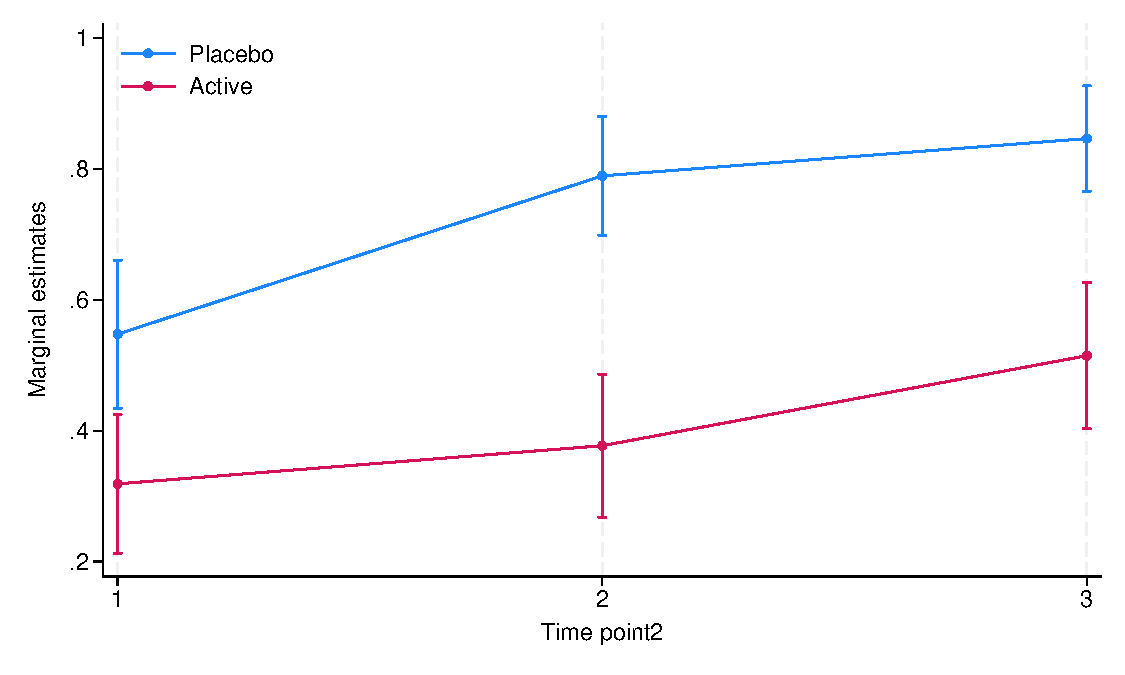
\includegraphics[width=0.85\linewidth]{stata/figures/cat_fig1} \caption{Margins plot by Stata}\label{fig:unnamed-chunk-1}
\end{figure}

The same in R using the \texttt{marginaleffects}-package:

\begin{Shaded}
\begin{Highlighting}[]
\NormalTok{mod }\OtherTok{\textless{}{-}}\NormalTok{ rct }\SpecialCharTok{\%\textgreater{}\%}
  \FunctionTok{filter}\NormalTok{(time }\SpecialCharTok{!=} \DecValTok{0}\NormalTok{) }\SpecialCharTok{\%\textgreater{}\%}
  \FunctionTok{glmer}\NormalTok{(catout }\SpecialCharTok{\textasciitilde{}}\NormalTok{ trt }\SpecialCharTok{+}\NormalTok{ time }\SpecialCharTok{+}\NormalTok{ trt}\SpecialCharTok{*}\NormalTok{time }\SpecialCharTok{+}\NormalTok{ site }\SpecialCharTok{+}\NormalTok{ covar }\SpecialCharTok{+}\NormalTok{ (}\DecValTok{1}\SpecialCharTok{|}\NormalTok{pid), }
        \AttributeTok{data =}\NormalTok{ ., }
        \AttributeTok{family =}\NormalTok{ binomial, }
        \AttributeTok{nAGQ =} \DecValTok{7}\NormalTok{)}

\NormalTok{pred }\OtherTok{\textless{}{-}}\NormalTok{ mod }\SpecialCharTok{\%\textgreater{}\%} 
  \FunctionTok{avg\_predictions}\NormalTok{(}\AttributeTok{variables =} \FunctionTok{list}\NormalTok{(}\AttributeTok{trt =} \FunctionTok{c}\NormalTok{( }\StringTok{"Placebo"}\NormalTok{, }\StringTok{"Active"}\NormalTok{), }\AttributeTok{time =} \FunctionTok{c}\NormalTok{(}\StringTok{"1"}\NormalTok{,}\StringTok{"2"}\NormalTok{, }\StringTok{"3"}\NormalTok{)), }\AttributeTok{type =} \StringTok{"response"}\NormalTok{) }
\end{Highlighting}
\end{Shaded}

\begin{verbatim}
Warning: For this model type, `marginaleffects` only takes into account the
  uncertainty in fixed-effect parameters. You can use the `re.form=NA`
  argument to acknowledge this explicitly and silence this warning.
\end{verbatim}

\begin{Shaded}
\begin{Highlighting}[]
\NormalTok{pred}
\end{Highlighting}
\end{Shaded}

\begin{verbatim}

 time     trt Estimate Std. Error     z Pr(>|z|)     S 2.5 % 97.5 %
    1 Placebo    0.548     0.0580  9.45   <0.001  67.9 0.434  0.662
    1 Active     0.318     0.0548  5.80   <0.001  27.2 0.210  0.425
    2 Placebo    0.791     0.0462 17.13   <0.001 216.1 0.701  0.882
    2 Active     0.376     0.0561  6.70   <0.001  35.5 0.266  0.486
    3 Placebo    0.848     0.0411 20.62   <0.001 311.3 0.767  0.929
    3 Active     0.515     0.0578  8.91   <0.001  60.8 0.402  0.628

Columns: trt, time, estimate, std.error, statistic, p.value, s.value, conf.low, conf.high 
Type:  response 
\end{verbatim}

The estimated marginal plot is then given by:

\begin{Shaded}
\begin{Highlighting}[]
\NormalTok{pred }\SpecialCharTok{\%\textgreater{}\%} 
  \FunctionTok{ggplot}\NormalTok{(}\FunctionTok{aes}\NormalTok{(time, estimate, }\AttributeTok{color=}\NormalTok{trt, }\AttributeTok{group=}\NormalTok{trt)) }\SpecialCharTok{+}
  \FunctionTok{geom\_point}\NormalTok{(}\AttributeTok{position =} \FunctionTok{position\_dodge}\NormalTok{(}\FloatTok{0.04}\NormalTok{)) }\SpecialCharTok{+}
  \FunctionTok{geom\_line}\NormalTok{() }\SpecialCharTok{+} 
  \FunctionTok{geom\_errorbar}\NormalTok{(}\FunctionTok{aes}\NormalTok{(}\AttributeTok{ymin =}\NormalTok{ conf.low, }\AttributeTok{ymax =}\NormalTok{ conf.high), }
                \AttributeTok{width=}\NormalTok{.}\DecValTok{2}\NormalTok{,}
                \AttributeTok{position =} \FunctionTok{position\_dodge}\NormalTok{(}\FloatTok{0.04}\NormalTok{)) }\SpecialCharTok{+} 
  \FunctionTok{ylab}\NormalTok{(}\StringTok{"Estimate"}\NormalTok{) }\SpecialCharTok{+}
  \FunctionTok{xlab}\NormalTok{(}\StringTok{"Time"}\NormalTok{) }\SpecialCharTok{+}
  \FunctionTok{theme\_classic}\NormalTok{() }\SpecialCharTok{+} 
  \FunctionTok{theme}\NormalTok{(}\AttributeTok{legend.position=}\FunctionTok{c}\NormalTok{(}\FloatTok{0.1}\NormalTok{,}\FloatTok{0.9}\NormalTok{)) }\SpecialCharTok{+}
  \FunctionTok{scale\_colour\_brewer}\NormalTok{(}\AttributeTok{palette =} \StringTok{"Set1"}\NormalTok{, }\AttributeTok{name =} \StringTok{"Treatment"}\NormalTok{)}
\end{Highlighting}
\end{Shaded}

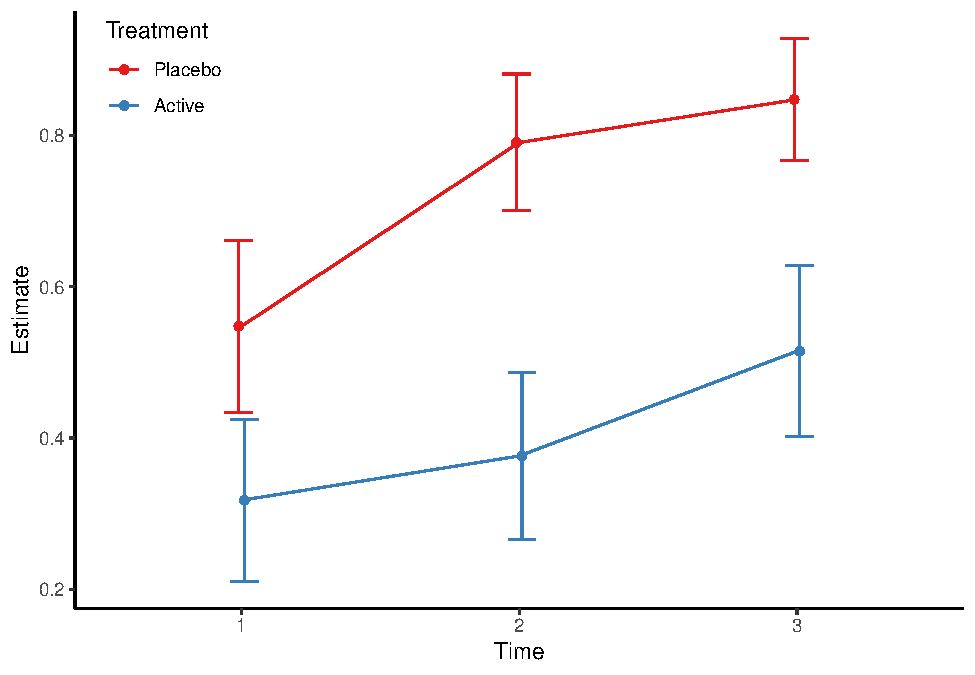
\includegraphics{rct-cookbook_files/figure-latex/rmixed4plot_02-1.pdf}

The treatment differences at different timepoints are then calculated with:

\begin{Shaded}
\begin{Highlighting}[]
\KeywordTok{use} \StringTok{"stata/rct"}\NormalTok{, }\KeywordTok{clear}
\KeywordTok{quietly}\NormalTok{ melogit catout i.trt i.site covar i.time i.trt\#i.time }\KeywordTok{if}\NormalTok{ time != 0 || pid:}
\NormalTok{margins time, }\KeywordTok{dydx}\NormalTok{(trt)}
\end{Highlighting}
\end{Shaded}

\begin{verbatim}
(all strata combined)



Average marginal effects                                   Number of obs = 294
Model VCE: OIM

Expression: Marginal predicted mean, predict()
dy/dx wrt:  1.trt

------------------------------------------------------------------------------
             |            Delta-method
             |      dy/dx   std. err.      z    P>|z|     [95% conf. interval]
-------------+----------------------------------------------------------------
0.trt        |  (base outcome)
-------------+----------------------------------------------------------------
1.trt        |
        time |
          1  |   -.228834    .079152    -2.89   0.004     -.383969   -.0736989
          2  |  -.4126365   .0726801    -5.68   0.000    -.5550869   -.2701861
          3  |  -.3319839    .070613    -4.70   0.000    -.4703829   -.1935849
------------------------------------------------------------------------------
Note: dy/dx for factor levels is the discrete change from the base level.
\end{verbatim}

In R this is done with the \texttt{marginaleffects}-package:

\begin{Shaded}
\begin{Highlighting}[]
\NormalTok{mod }\OtherTok{\textless{}{-}}\NormalTok{ rct }\SpecialCharTok{\%\textgreater{}\%}
  \FunctionTok{filter}\NormalTok{(time }\SpecialCharTok{!=} \DecValTok{0}\NormalTok{) }\SpecialCharTok{\%\textgreater{}\%}
  \FunctionTok{glmer}\NormalTok{(catout }\SpecialCharTok{\textasciitilde{}}\NormalTok{ trt }\SpecialCharTok{+}\NormalTok{ time }\SpecialCharTok{+}\NormalTok{ trt}\SpecialCharTok{*}\NormalTok{time }\SpecialCharTok{+}\NormalTok{ site }\SpecialCharTok{+}\NormalTok{ covar }\SpecialCharTok{+}\NormalTok{ (}\DecValTok{1}\SpecialCharTok{|}\NormalTok{pid), }
        \AttributeTok{data =}\NormalTok{ ., }
        \AttributeTok{family =}\NormalTok{ binomial, }
        \AttributeTok{nAGQ =} \DecValTok{7}\NormalTok{)}

\NormalTok{mod }\SpecialCharTok{\%\textgreater{}\%}
  \FunctionTok{avg\_comparisons}\NormalTok{(}\AttributeTok{variables =} \FunctionTok{list}\NormalTok{(}\AttributeTok{trt =} \FunctionTok{c}\NormalTok{(}\StringTok{"Active"}\NormalTok{, }\StringTok{"Placebo"}\NormalTok{)), }\AttributeTok{by =} \StringTok{"time"}\NormalTok{, }\AttributeTok{type =} \StringTok{"response"}\NormalTok{, }\AttributeTok{re.form =} \ConstantTok{NA}\NormalTok{)}
\end{Highlighting}
\end{Shaded}

\begin{verbatim}

 Term                     Contrast time Estimate Std. Error    z Pr(>|z|)    S
  trt mean(Placebo) - mean(Active)    1    0.230     0.0797 2.89  0.00386  8.0
  trt mean(Placebo) - mean(Active)    2    0.414     0.0728 5.69  < 0.001 26.2
  trt mean(Placebo) - mean(Active)    3    0.333     0.0704 4.73  < 0.001 18.7
  2.5 % 97.5 %
 0.0741  0.387
 0.2717  0.557
 0.1947  0.471

Columns: term, contrast, time, estimate, std.error, statistic, p.value, s.value, conf.low, conf.high, predicted_lo, predicted_hi, predicted 
Type:  response 
\end{verbatim}

We see the results are slightly different to the Stata results, but the differences are small.

\chapter{Time to event analyses}\label{time-to-event-analyses}

To be done

\chapter{Sample size calculations}\label{sample-size-calculations}

To be done

  \bibliography{packages.bib}

\end{document}
